\section{ALGUNS SUBCAPÍTULOS DA TEORIA DE GRAFOS}
\subsection{Grafos simples e multigrafo}
\noindent{ - \underline{Grafo simples}, onde entre dois vértices estão conectados por apenas uma aresta. Isto é válido para todos os vértices do grafo.}
\begin{figure}[h]
    \centering
    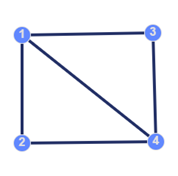
\includegraphics[width=0.2\textwidth]{imgs/Figura3}
    \caption{Exemplo de grafo simples\label{fig:imagem3}}
\end{figure}
\linebreak
- \underline{Multigrafo}, no caso de terem várias arestas a conectar os mesmos dois vértices, ou no caso de um vértice possuir um lacete, ou seja, uma “aresta” a ligar esse mesmo vértice nas duas extremidades.
\begin{figure}[h]
    \centering
    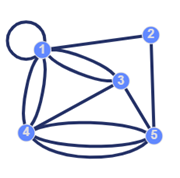
\includegraphics[width=0.2\textwidth]{imgs/Figura4}
    \caption{Exemplo de multigrafo com lacete\label{fig:imagem4}}
\end{figure}
\linebreak
\flushright\scriptsize{(Nas companhias aéreas os passageiros detestam lacetes.\\O avião descola do aeroporto e pouco\\depois aterra no mesmo novamente!)}
\subsection{Digrafos ou grafos orientados}
São grafos que apresentam na sua totalidade arestas orientadas, mais conhecidas como arcos.
\linebreak
\begin{figure}[h]
    \centering
    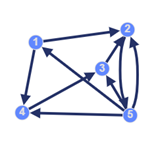
\includegraphics[width=0.2\textwidth]{imgs/Figura5}
    \caption{Exemplo de multigrafo com lacete\label{fig:imagem5}}
\end{figure}

\subsection{Grafo Parcial e Subgrafo gerado de um dado grafo}
